\documentclass[11pt,openany]{article}

\usepackage{mathtools, commath}
% Packages for formatting
\usepackage[margin=1in]{geometry}
\usepackage{fancyhdr}
\usepackage{enumerate}
\usepackage{graphicx}
\usepackage{kotex}
\usepackage{arydshln} % Include this package
\usepackage{bbding}
\usepackage{amsmath}
\usepackage{amsthm}
\usepackage[dvipsnames,table]{xcolor}
\usepackage{amssymb, amsfonts}
\usepackage{wasysym}
\usepackage{footnote}
\usepackage{tablefootnote}
\usepackage{arydshln} % Include this package
% Fonts
\usepackage[T1]{fontenc}
\usepackage[utf8]{inputenc}
\usepackage{newpxtext,newpxmath}
\usepackage{sectsty}

% Define colors
\definecolor{TealBlue1}{HTML}{0077c2}
\definecolor{TealBlue2}{HTML}{00a5e6}
\definecolor{TealBlue3}{HTML}{b3e0ff}
\definecolor{TealBlue4}{HTML}{00293c}
\definecolor{TealBlue5}{HTML}{e6f7ff}

\definecolor{thmcolor}{RGB}{231, 76, 60}
\definecolor{defcolor}{RGB}{52, 152, 219}
\definecolor{lemcolor}{RGB}{155, 89, 182}
\definecolor{corcolor}{RGB}{46, 204, 113}
\definecolor{procolor}{RGB}{241, 196, 15}

\usepackage{color,soul}
\usepackage{soul}
\newcommand{\mathcolorbox}[2]{\colorbox{#1}{$\displaystyle #2$}}
\usepackage{cancel}
\newcommand\crossout[3][black]{\renewcommand\CancelColor{\color{#1}}\cancelto{#2}{#3}}
\newcommand\ncrossout[2][black]{\renewcommand\CancelColor{\color{#1}}\cancel{#2}}

\usepackage{hyperref}
\usepackage{booktabs}

% Chapter formatting
\definecolor{titleTealBlue}{RGB}{0,53,128}
\usepackage{titlesec}
\titleformat{\section}
{\normalfont\sffamily\Large\bfseries\color{titleTealBlue!100!gray}}{\thesection}{1em}{}
\titleformat{\subsection}
{\normalfont\sffamily\large\bfseries\color{titleTealBlue!50!gray}}{\thesubsection}{1em}{}

%Tcolorbox
\usepackage[most]{tcolorbox}
\usepackage{multirow}
\usepackage{multicol}

\usepackage[linesnumbered,ruled]{algorithm2e}
\usepackage{algpseudocode}
\usepackage{setspace}
\SetKwComment{Comment}{/* }{ */}
\SetKwProg{Fn}{Function}{:}{end}
\SetKw{End}{end}
\SetKw{DownTo}{downto}

% Define a new environment for algorithms without line numbers
\newenvironment{algorithm2}[1][]{
	% Save the current state of the algorithm counter
	\newcounter{tempCounter}
	\setcounter{tempCounter}{\value{algocf}}
	% redefine the algorithm numbering (remove prefix)
	\renewcommand{\thealgocf}{}
	\begin{algorithm}
	}{
	\end{algorithm}
	% Restore the algorithm counter state
	\setcounter{algocf}{\value{tempCounter}}
}

\usepackage{adjustbox}
% Header and footer formatting
\pagestyle{fancy}
\fancyhead{}
\fancyhf{}
\rhead{\textcolor{TealBlue2}{\large\textbf{기대수(기초부터 대학원 수학까지 시리즈) 3기}}}%\rule{3cm}{0.4pt}}
\lhead{\textcolor{TealBlue2}{\large\textbf{수학의 즐거움, Enjoying Math}}}
% Define footer
%\newcommand{\footer}[1]{
%\begin{flushright}
%	\vspace{2em}
%	\includegraphics[width=2.5cm]{school_logo.jpg} \\
%	\vspace{1em}
%	\textcolor{TealBlue2}{\small\textbf{#1}}
%\end{flushright}
%}
%\rfoot{\large Department of Information Security, Cryptogrphy and Mathematics, Kookmin Uni.\includegraphics[height=1.5cm]{school_logo.jpg}}
\fancyfoot{}
\fancyfoot[C]{-\thepage-}

\usepackage{tcolorbox}
\tcbset{colback=white, arc=5pt}

\definecolor{axiomcolor}{HTML}{a88bfa}
\definecolor{defcolor}{RGB}{52, 152, 219}
\definecolor{procolor}{RGB}{241, 196, 15}
\definecolor{thmcolor}{RGB}{231, 76, 60}
\definecolor{lemcolor}{RGB}{155, 89, 182}
\definecolor{corcolor}{RGB}{46, 204, 113}
\definecolor{execolor}{RGB}{90, 128, 127}

% Define a new command for the custom tcolorbox
\newcommand{\axiombox}[2][]{%
	\begin{tcolorbox}[colframe=axiomcolor, title={\color{white}\bfseries #1}]
		#2
	\end{tcolorbox}
}

\newcommand{\defbox}[2][]{%
	\begin{tcolorbox}[colframe=defcolor, title={\color{white}\bfseries #1}]
		#2
	\end{tcolorbox}
}

\newcommand{\lembox}[2][]{%
	\begin{tcolorbox}[colframe=lemcolor, title={\color{white}\bfseries #1}]
		#2
	\end{tcolorbox}
}

\newcommand{\probox}[2][]{%
	\begin{tcolorbox}[colframe=procolor, title={\color{white}\bfseries #1}]
		#2
	\end{tcolorbox}
}

\newcommand{\thmbox}[2][]{%
	\begin{tcolorbox}[colframe=thmcolor, title={\color{white}\bfseries #1}]
		#2
	\end{tcolorbox}
}

\newcommand{\corbox}[2][]{%
	\begin{tcolorbox}[colframe=corcolor, title={\color{white}\bfseries #1}]
		#2
	\end{tcolorbox}
}



\usepackage{amsthm}

% Define custom theorem styles
\newtheoremstyle{dotless} % Name of the style
{3pt} % Space above
{3pt} % Space below
{\itshape} % Body font
{} % Indent amount
{\bfseries} % Theorem head font
{} % Punctuation after theorem head
{2.5mm} % Space after theorem head
{} % Theorem head spec

\newtheoremstyle{definitionstyle} % Name of the style
{3pt} % Space above
{3pt} % Space below
{} % Body font
{} % Indent amount
{\bfseries} % Theorem head font
{.} % Punctuation after theorem head
{2.5mm} % Space after theorem head
{} % Theorem head spec

% Applying custom styles
\theoremstyle{dotless}
\newtheorem{theorem}{Theorem} % Theorem environment with section-wise numbering
\newtheorem{proposition}[theorem]{Proposition} % Theorem environment with section-wise numbering
\newtheorem{lemma}[theorem]{Lemma} % Lemma shares the counter with theorem
\newtheorem{corollary}[theorem]{Corollary} % Corollary shares the counter with theorem

\theoremstyle{definitionstyle}
\newtheorem*{observation}{\textcolor{Magenta}{Observation}}
\newtheorem{definition}{Definition} % Definition shares the counter with theorem
\newtheorem{example}{Example} % Example shares the counter with theorem
\newtheorem{exercise}{Exercise} % Example shares the counter with theorem
\newtheorem{remark}{Remark} % Remark shares the counter with theorem
\newtheorem*{note}{Note}

\newtheorem*{definition*}{Definition} % Definition shares the counter with theorem
\newtheorem*{example*}{Example} % Example shares the counter with theorem
\newtheorem*{exercise*}{\textcolor{violet}{Exercise}} % Example shares the counter with theorem
\newtheorem*{remark*}{Remark} % Remark shares the counter with theorem


\usepackage{tikz}
\usepackage{tikz-cd}
\usepackage{tikz-3dplot}
\usepackage{pgfplots}
\pgfplotsset{compat=newest} % Adjust to your version of pgfplots
\def\Circlearrowleft{\ensuremath{%
		\rotatebox[origin=c]{180}{$\circlearrowleft$}}}
\def\Circlearrowright{\ensuremath{%
		\rotatebox[origin=c]{180}{$\circlearrowright$}}}
\def\CircleArrowleft{\ensuremath{%
		\reflectbox{\rotatebox[origin=c]{180}{$\circlearrowleft$}}}}
\def\CircleArrowright{\ensuremath{%
		\reflectbox{\rotatebox[origin=c]{180}{$\circlearrowright$}}}}
\usetikzlibrary{
	3d, % For 3D drawing
	angles,
	arrows,
	arrows.meta,
	backgrounds,
	bending,
	calc,
	decorations.pathmorphing,
	decorations.pathreplacing,
	decorations.markings,
	fit,
	matrix,
	patterns,
	patterns.meta,
	positioning,
	quotes,
	shadows,
	shapes,
	shapes.geometric,
	tikzmark
}
\tikzset{
	% single mid‐path arrow
	mid arrow/.style={
		decoration={
			markings,
			mark=at position 0.5 with {\arrow{Stealth[scale=1.2]}}
		},
		postaction={decorate},
	},
	% style for field arrows
	field arrow/.style={
		-{Stealth[scale=1.0]},
		thick,
		blue!70!black,
	},
}
\newcommand{\ie}{\textnormal{i.e.}}
\newcommand{\rsa}{\mathsf{RSA}}
\newcommand{\rsacrt}{\mathsf{RSA}\textendash\mathsf{CRT}}
\newcommand{\inv}[1]{#1^{-1}}

%New Command
%\newcommand{\set}[1]{\left\{#1\right\}}
\newcommand{\N}{\mathbb{N}}
\newcommand{\Z}{\mathbb{Z}}
\newcommand{\Q}{\mathbb{Q}}
\newcommand{\R}{\mathbb{R}}
\newcommand{\cR}{\mathcal{R}}
\newcommand{\C}{\mathbb{C}}
\newcommand{\F}{\mathbb{F}}
\newcommand{\nbhd}{\mathcal{N}}
\newcommand{\Log}{\operatorname{Log}}
\newcommand{\Arg}{\operatorname{Arg}}
\newcommand{\pv}{\operatorname{P.V.}}

\newcommand{\of}[1]{\left( #1 \right)} 
%\newcommand{\abs}[1]{\left\lvert #1 \right\rvert}
%\newcommand{\norm}[1]{\left\| #1 \right\|}

\newcommand{\sol}{\textcolor{magenta}{\bf Sol}}
\newcommand{\conjugate}[1]{\overline{#1}}

\newcommand{\res}{\operatorname{res}}
\DeclareMathOperator*{\Res}{\operatorname{Res}}

%\renewcommand{\Re}{\operatorname{Re}}
%\renewcommand{\Im}{\operatorname{Im}}

\newcommand{\cyclic}[1]{\langle #1 \rangle}
\newcommand{\uniform}{\overset{\$}{\leftarrow}}
\newcommand{\xmark}{\textcolor{red}{\XSolidBrush}}
\newcommand{\vmark}{\textcolor{green!75!black}{\CheckmarkBold}}

\newcommand{\gen}[1]{\langle #1 \rangle}
\newcommand{\Gen}[1]{\left\langle #1 \right\rangle}

\newcommand{\img}[1]{\text{Img}(#1)}
\newcommand{\Img}[1]{\text{Img}\left(#1\right)}
\newcommand{\preimg}[1]{\text{Img}^{-1}(#1)}
\newcommand{\Preimg}[1]{\text{Img}^{-1}\left(#1\right)}

\newcommand{\relation}{\mathrel{\mathcal{R}}}
\newcommand{\injection}{\rightarrowtail}
\newcommand{\surjection}{\twoheadrightarrow}
\newcommand{\id}{\textnormal{id}}

\newcommand{\eqclass}[1]{\left[#1\right]}

% Define custom colors for O and X
\newcommand{\yes}{\textcolor{blue}{\bf \fullmoon}}
\newcommand{\no}{\textcolor{red}{\bf \texttimes}}

\DeclarePairedDelimiter\ceil{\lceil}{\rceil}
\DeclarePairedDelimiter\floor{\lfloor}{\rfloor}
%\renewcommand{\floor}[#1]{\lfloor #1\rfloor}
%\newcommand{\Floor}[#1]{\left\lfloor #1\right\rfloor}
%\newcommand{\ceil}[#1]{\lceil #1\rceil}
%\newcommand{\Ceil}[#1]{\left\lceil #1\right\rceil}

\newcommand{\topology}{\mathscr{T}}
\newcommand{\sequence}[1]{\langle #1\rangle}
\renewcommand{\vec}[1]{\mathbf{#1}}
\setstretch{1.25}

%\usepackage{background}
%\backgroundsetup{
%	scale=3,
%	color=gray!20,
%	opacity=0.3,
%	angle=45,
%	contents={\Huge \sffamily Ji, Yong-hyeon}
%}
\begin{document}
\pagenumbering{arabic}
\begin{center}
	\huge\textbf{Linear Algebra I}\\
	\vspace{0.5em}
	\large{Ji, Yong-hyeon}\\
%	\large{\ttfamily \url{https://github.com/Hacker-Code-J}}\\
	\vspace{0.5em}
	\normalsize{\today}\\
\end{center}

\noindent 
We cover the following topics in this note.
\begin{itemize}
	\item Linear Combination, Spanning Set
	\item Linearly Independent and Dependent
	\item (Hamel) Basis
	\item Partial Order; POSET
	\item Total Order (Linear Order); TOSET
	\item Maximal, Minimal, Hasse Diagram
	\item Chain, Zorn's Lemma
	\item Hamel Basis Theorem (Existence of Basis)
	\item Invariance of Basis Cardinality; Dimension of Vector Space
\end{itemize}
\hrule\vspace{12pt}
%\tableofcontents
%\newpage
\begin{center}
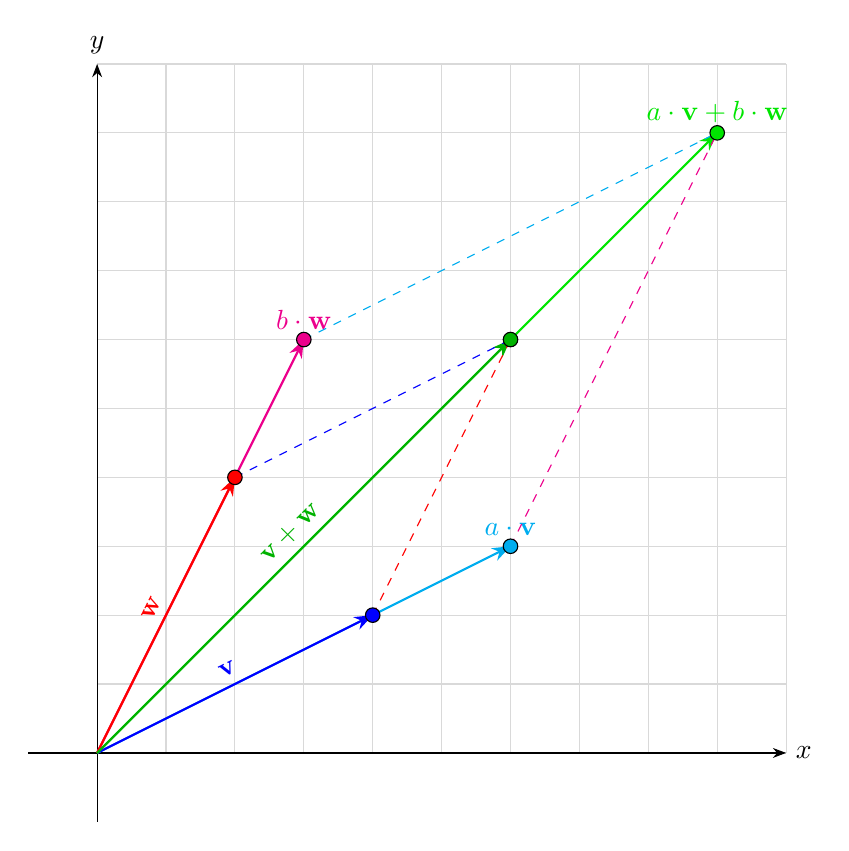
\begin{tikzpicture}[scale=1.75, >=Stealth]
	\foreach \x in {0,.5,...,5}
	\draw[gray!30] (\x,0) -- (\x,5);
	\foreach \y in {0,.5,...,5}
	\draw[gray!30] (0,\y) -- (5,\y);
	
	\draw[->] (-0.5,0) -- (5,0) node[right] {$x$};
	\draw[->] (0,-0.5) -- (0,5) node[above] {$y$};
	\draw[->, thick, cyan] (0,0) -- (3,1.5) node[above] {$a\cdot\vec{v}$};
	\draw[->, thick, blue] (0,0) -- (2,1) node[midway, above, sloped] {$\vec{v}$};
	\draw[->, thick, magenta] (0,0) -- (1.5,3) node[above] {$b\cdot\vec{w}$};
	\draw[->, thick, red] (0,0) -- (1,2) node[midway, above, sloped] {$\vec{w}$};
	\draw[->, thick, green!90!black] (0,0) -- (4.5,4.5) node[above, sloped] {$a\cdot\vec{v}+b\cdot\vec{w}$};
	\draw[->, thick, green!70!black] (0,0) -- (3,3) node[midway, above, sloped] {$\vec{v}+\vec{w}$};
	\draw[dashed, red] (2,1) -- (3,3);
	\draw[dashed, blue] (1,2) -- (3,3);
	\draw[dashed, magenta] (3,1.5) -- (4.5,4.5);
	\draw[dashed, cyan] (1.5,3) -- (4.5,4.5);
	\draw[fill=red] (1,2) circle (1.5pt);
	\draw[fill=blue] (2,1) circle (1.5pt);
	\draw[fill=green!70!black] (3,3) circle (1.5pt);
	\draw[fill=magenta] (1.5,3) circle (1.5pt);
	\draw[fill=cyan] (3,1.5) circle (1.5pt);
	\draw[fill=green!90!black] (4.5,4.5) circle (1.5pt);
\end{tikzpicture}
\end{center}

\newpage
\defbox[Vector Space]{\begin{definition*}
Let \( F \) be a field. A \hl{\textbf{vector space}} over \( F \) (or a $F$-vector space) is a structure \((V, +, \cdot)\) satisfying the following axioms:
\begin{enumerate}[(i)]
	\item \((V, +)\) is an abelian group with additive identity \( \vec{0} \in V \).
	\item Define \emph{scalar multiplication} as the function\quad $\cdot:F\times V\to V$,\quad $(a,\vec{v})\mapsto a\cdot\vec{v}$. 
%	\[
%	\fullfunction{\cdot }{F\times V}{V}{(a,\vec{v})}{a\cdot\vec{v}}.
%	\]
	\item (Compatibility) For all $a,b\in F$ and $\vec{v},\vec{w}\in V$,
	\begin{enumerate}[(a)]
		\item $a \cdot (\vec{v}+\vec{w}) = a \cdot \vec{v} + a \cdot \vec{w}$.\hfill(Distributivity over vector addition)
		\item $(a+b) \cdot \vec{v} = a \cdot \vec{v} + b \cdot \vec{v}$.\hfill(Distributivity over field addition)
		\item $a \cdot (b \cdot \vec{v}) = (a b) \cdot \vec{v}$.\hfill(Associativity of scalar multiplication)
		\item $1_F \cdot \vec{v} = \vec{v}$.\hfill(Identity of scalar multiplication)
		\item[\textcolor{gray!50}{(e)}] \color{gray!50} $0_F \cdot \vec{v} = \vec{0}$.
	\end{enumerate}
\end{enumerate} 
\end{definition*}}

%-------------------------------------------------------------------
% Geometric illustration: Vector Addition via the Parallelogram Rule
%-------------------------------------------------------------------
\begin{center}
\begin{minipage}{.49\textwidth}\centering
%-------------------------------------------------------------------
% 1. Distributivity over Vector Addition:
%    a(\vec{u}+\vec{v}) = a\vec{u} + a\vec{v}
%-------------------------------------------------------------------
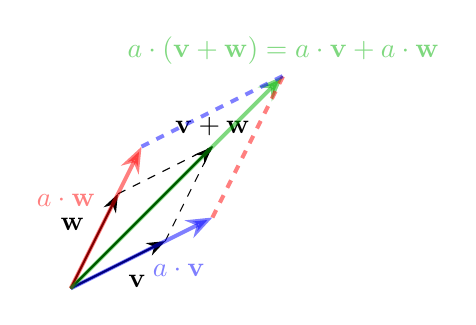
\begin{tikzpicture}[scale=1.2, >=Stealth]
	\draw[->, thick] (0,0) -- (1,.5) node[midway, below right] {$\vec{v}$};
	\draw[->, thick] (0,0) -- (.5,1) node[midway, above left] {$\vec{w}$};
	\draw[->, thick] (0,0) -- (1.5,1.5) node[above] {$\vec{v}+\vec{w}$};
	\draw[dashed] (1,.5) -- (1.5,1.5);
	\draw[dashed] (.5,1) -- (1.5,1.5);
	
	\draw[->, line width=.5mm, blue, opacity=.5] (0,0) -- (1.5,.75) node[midway, below right] {$a\cdot \vec{v}$};
	\draw[->, line width=.5mm, red, opacity=.5] (0,0) -- (.75,1.5) node[midway, above left] {$a\cdot \vec{w}$};
	\draw[->, line width=.5mm, green!70!black, opacity=.5] (0,0) -- (2.25,2.25) node[above] {$a\cdot (\vec{v}+\vec{w})=a\cdot\vec{v}+a\cdot\vec{w}$};
	\draw[dashed, line width=.5mm, red, opacity=.5] (1.5,.75) -- (2.25,2.25);
	\draw[dashed, line width=.5mm, blue, opacity=.5] (.75,1.5) -- (2.25,2.25);
\end{tikzpicture}
\end{minipage}
\begin{minipage}{.49\textwidth}\centering
%-------------------------------------------------------------------
% 2. Distributivity over Field Addition:
%    (a+b)\vec{v} = a\vec{v} + b\vec{v}
%-------------------------------------------------------------------
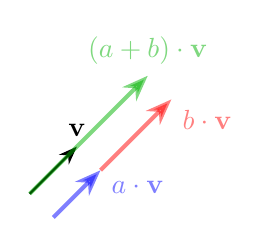
\begin{tikzpicture}[scale=1.2, >=Stealth]
	\draw[->, thick] (0,0) -- (.5,.5) node[above] {$\vec{v}$};
	\draw[->, line width=.5mm, blue, opacity=.5] (0+.25,0-.25) -- (.5+.25,.5-.25) node[below right] {$a\cdot\vec{v}$};
	\draw[->, line width=.5mm, red, opacity=.5] (.5+.25,.5-.25) -- (1.25+.25,1.25-.25) node[below right] {$b\cdot\vec{v}$};
	\draw[->, line width=.5mm, green!70!black, opacity=.5] (0,0) -- (1.25,1.25) node[above] {$(a+b)\cdot\vec{v}$};
\end{tikzpicture}
\end{minipage}
\end{center}
\begin{center}
\begin{minipage}{.49\textwidth}\centering
%-------------------------------------------------------------------
% 3. Associativity of Scalar Multiplication: 
%    a (b\vec{v}) = (ab)\vec{v}
%-------------------------------------------------------------------
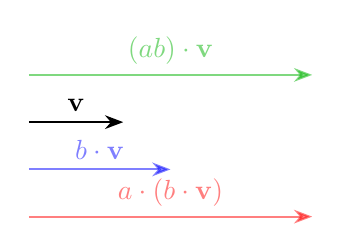
\begin{tikzpicture}[scale=1.2, >=Stealth]
	\draw[->, thick] (0,0) -- (1,0) node[midway, above] {$\vec{v}$};
	\draw[->, thick, blue, opacity=.5] (0,-.5) -- (1.5,-.5) node[midway, above] {$b\cdot \vec{v}$};
	\draw[->, thick, red, opacity=.5] (0,-1) -- (3,-1) node[midway, above] {$a\cdot (b\cdot \vec{v})$};
	\draw[->, thick, green!70!black, opacity=.5] (0,.5) -- (3,.5) node[midway, above] {$(ab)\cdot \vec{v}$};
\end{tikzpicture}
\end{minipage}
\begin{minipage}{.49\textwidth}\centering
%-------------------------------------------------------------------
% 4. Identity of Scalar Multiplication:
%    1\vec{v} = \vec{v}
%-------------------------------------------------------------------
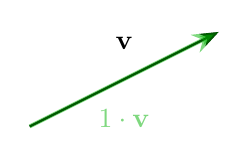
\begin{tikzpicture}[scale=1.2, >=Stealth]
	\coordinate (O) at (0,0);
	% Define an arbitrary vector v.
	\coordinate (V) at (2,1);
	\draw[->, thick] (O) -- (V) node[midway, above, yshift=.25cm] {$\vec{v}$};
	
	% The scaling by 1 leaves v unchanged.
	\coordinate (OneV) at ($ (O)!{1}!(V) $);
	\draw[->, line width=.5mm, green!70!black, opacity=.5] (O) -- (OneV) node[midway, below, yshift=-.25cm] {$1\cdot\vec{v}$};
\end{tikzpicture}
\end{minipage}
\end{center}
\vspace{40pt}
\begin{remark*}
Consider a vector space $V$ over a field $F$. Let $\vec{v}\in V$. Since $0_F = 0_F + 0_F$ (over $F$), we have \[
0_F \cdot \vec{v}=(0_F+0_F)\cdot \vec{v}\overset{\text{(iii)-(b)}}{=}0_F\cdot \vec{v}+ 0_F\cdot \vec{v}.
\] Then  \begin{align*}
0_F\cdot \vec{v}\textcolor{red}{\;+\; (-\ 0_F\cdot \vec{v})}&=0_F\cdot \vec{v}+ 0_F\cdot \vec{v}\textcolor{red}{\;+\; (-\ 0_F\cdot \vec{v})},\\
\vec{0}&=0_F\cdot \vec{v}+\vec{0},\\
\vec{0}&=0_F\cdot \vec{v}.
\end{align*}
\end{remark*}

\newpage
\defbox[Linear Combination and Spanning Set]{\begin{definition*}
Let $V$ be a vector space over a field $F$, and let $S$ be a subset of $V$

\begin{enumerate}[(1)]
	\item A vector $\vec{v}\in V$ is called a \hl{\textbf{linear combination}} of elements of $S$ if there exists finite number of vectors $\vec{b}_1,\vec{b}_2,\dots,\vec{b}_n\in S$ and scalars $a_1,a_2,\dots, a_n\in F$ such that \[
	\vec{v}=a_1\vec{b}_1+a_2\vec{b}_2+\cdots+a_n\vec{b}_n=\sum_{i=1}^{n}a_i\vec{b}_i.
	\]
	\item The \hl{\textbf{subspace spanned by $S$} (or \textbf{spanning set} $S$)}, denoted by $\Span(S)$, is the set of all finite linear combinations of elements of $S$: \begin{align*}
		\Span(S)&=\set{a_1\vec{b}_1+a_2\vec{b}_2+\cdots +a_n\vec{b}_n\mid a_i\in F, \vec{b}_i\in S\ \text{for all}\ i=1,2,\dots,n} \\
		&=\set{\sum_{i=1}^{n}a_i\vec{b}_i\ \bigg|\ a_i\in F, \vec{b}_i\in S\ \text{for all}\ i=1,2,\dots,n} \\
	\end{align*}
\end{enumerate}
\end{definition*}}
\begin{example*}
Consider the vector space $\R^2$ and the subset \[
S=\set{\vec{b}_1,\vec{b}_2}\quad\text{with}\quad \vec{b}_1=(2,1)\ \text{and}\ \vec{b}_2=(1,3).
\] 
\begin{center}
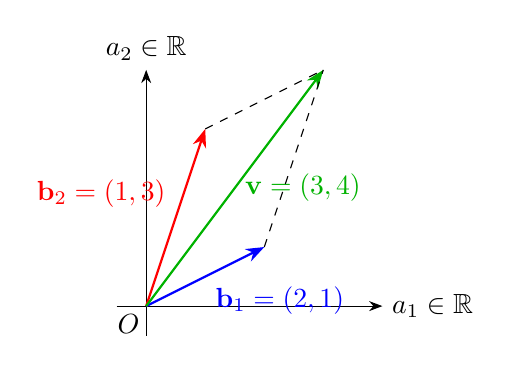
\begin{tikzpicture}[scale=0.75, >=Stealth]
	% Draw coordinate axes
	\draw[->] (-.5,0) -- (4,0) node[right] {$a_1\in\R$};
	\draw[->] (0,-.5) -- (0,4) node[above] {$a_2\in\R$};
	
	% Define vectors from S: v1 = (2,1) and v2 = (1,3)
	\coordinate (v1) at (2,1);
	\coordinate (v2) at (1,3);
	
	% Draw the vectors (elements of S)
	\draw[->, thick, blue] (0,0) -- (v1) node[midway, below right] {$\vec{b}_1=(2,1)$};
	\draw[->, thick, red] (0,0) -- (v2) node[midway, above left] {$\vec{b}_2=(1,3)$};
	
	% Illustrate a linear combination: e.g., 1*v1 + 1*v2 = (3,4)
	\coordinate (v12) at (3,4);
	\draw[->, thick, green!70!black] (0,0) -- (v12) node[midway, right] {$\vec{v}=(3,4)$};
	
	% Draw the parallelogram for visualizing the linear combination
	\draw[dashed] (v1) -- (v12);
	\draw[dashed] (v2) -- (v12);
	
	% Label the origin
	\node at (-0.3,-0.3) {$O$};
\end{tikzpicture}
\end{center}
\begin{itemize}
	\item A vector $\vec{v}=(3,4)\in\R^2$ is a linear combination of $\vec{b}_1$ and $\vec{b}_2$ since \[
	\vec{v}=(3,4)=(2\cdot 1+1,1+3\cdot 1)=1\cdot(2,1)+1\cdot(1,3),\quad\ie,\quad\vec{v}=\begin{bmatrix}
		3\\ 4
	\end{bmatrix}=\begin{bmatrix}
	2 & 1 \\ 1 & 3
\end{bmatrix}\begin{bmatrix}
1\\ 1
\end{bmatrix}.
	\]
	\item Since $\vec{b}_1$ and $\vec{b}_2$ are not colinear (they are lineary independent), every vector in $\R^2$ can be expressed in the form $(2a_1+a_2,a_1+3a_2)$ for some $a_1,a_2\in\R$. Hence \[
	\Span(S)=\R^2.
	\]
\end{itemize}
\end{example*}

\newpage
\defbox[Linearly Independent and Dependent]{\begin{definition*}
Let $V$ be a vector space over a field $F$ and let $S\subseteq V$. 
\begin{enumerate}[(1)]
	\item The set $S$ said to be \hl{\textbf{linearly independent}} if, for any finite collection of distinct vectors $\vec{b}_1,\vec{b}_2,\dots,\vec{b}_n\in S$ and any scalars $a_1,a_2,\dots, a_n\in F$, \[
	a_1\vec{b}_1+a_2\vec{b}_2+\cdots+a_n\vec{b}_n=\vec{0}\implies
	a_1=a_2=\cdots=a_n=0.
	\]
	\item The set $S$ is said to be \hl{\textbf{linearly dependent}} (\ie, not linearly independent) if there exists finitely many distinct vectors $\vec{b}_1,\vec{b}_2,\cdots,\vec{b}_n\in S$ and scalars $a_1,a_2,\dots,a_n\in F$, not all zeros, such that \[
	a_1\vec{b}_1+a_2\vec{b}_2+\cdots +a_n\vec{b}_n=\vec{0}.
	\] 
\end{enumerate}
\end{definition*}}
\begin{remark*}
In (2), suppose that $a_1\neq 0$, Then \[
a_1\vec{b}_1=-a_2\vec{b}_2-\cdots-a_n\vec{b}_n\iff \vec{b}_1=-a_1^{-1}(a_2\vec{b}_2+\cdots+a_n\vec{b}_n).
\] That is, a set $S$ is linearly dependent if at least one vector in $S$ can be expressed as a linear combination of the others.
\end{remark*}
\vfill
\begin{example*}
\ \begin{center}
\begin{minipage}{.48\textwidth}\centering
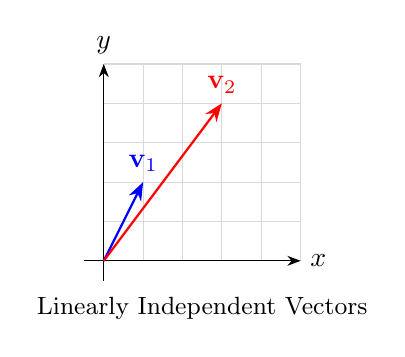
\begin{tikzpicture}[scale=.5, >=Stealth]
	% Optional: Draw a grid or dots to emphasize the plane
	\foreach \x in {0,...,5}
	\draw[gray!30] (\x,0) -- (\x,5);
	\foreach \y in {0,...,5}
	\draw[gray!30] (0,\y) -- (5,\y);
	
	% Draw coordinate axes
	\draw[->] (-.5,0) -- (5,0) node[right] {$x$};
	\draw[->] (0,-.5) -- (0,5) node[above] {$y$};
	
	% Define vectors
	\coordinate (v1) at (1,2);
	\coordinate (v2) at (3,4);
	
	% Draw vectors with arrows
	\draw[->, thick, blue] (0,0) -- (v1) node[above] {$\vec{v}_1$};
	\draw[->, thick, red] (0,0) -- (v2) node[above] {$\vec{v}_2$};
	\node at (2.5,-1.2) {\small Linearly Independent Vectors};
\end{tikzpicture}
\end{minipage}
\begin{minipage}{.48\textwidth}\centering
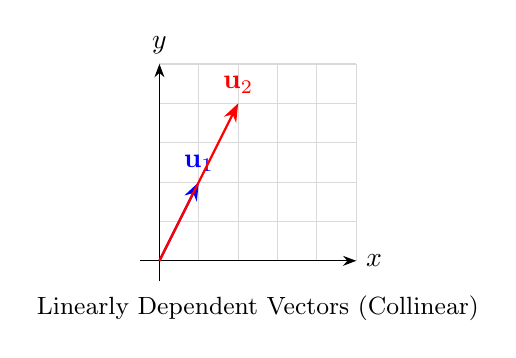
\begin{tikzpicture}[scale=.5, >=Stealth]
	\foreach \x in {0,...,5}
	\draw[gray!30] (\x,0) -- (\x,5);
	\foreach \y in {0,...,5}
	\draw[gray!30] (0,\y) -- (5,\y);
	% Draw coordinate axes
	\draw[->] (-.5,0) -- (5,0) node[right] {$x$};
	\draw[->] (0,-.5) -- (0,5) node[above] {$y$};
	
	% Define vectors: u1 and its multiple u2 = 2*u1
	\coordinate (u1) at (1,2);
	\coordinate (u2) at (2,4);
	
	% Draw vectors with arrows
	\draw[->, thick, blue] (0,0) -- (u1) node[above] {$\vec{u}_1$};
	\draw[->, thick, red] (0,0) -- (u2) node[above] {$\vec{u}_2$};
	
	
	% Caption for the illustration
	\node at (2.5,-1.2) {\small Linearly Dependent Vectors (Collinear)};
\end{tikzpicture}
\end{minipage}
\end{center}\begin{itemize}
\item The vectors $\vec{v}_1=(1,2)$ and $\vec{v}_2=(3,4)$ are linearly independent because the only solution to \[
a\vec{v}_1+b\vec{v}_2=\vec{0}
\] is $a=0$ and $b=0$.

\item The vectors $\vec{u}_1=(1,2)$ and $\vec{u}_2=(2,4)$ are linearly dependent because $\vec{u}_2$ is a multiple of $\vec{u}_1$; nontrivial solutions exist for \[
a\vec{u}_1+b\vec{u}_2=\vec{0}.
\]
\end{itemize}
\end{example*}

\newpage
\begin{remark*}
	In any vector space $V$, we can always find a subset of $S$ such that \[
	\Span(S)=V.
	\] For instance, taking $S=V$ gives $\Span(S)=V$. Since $S=V$, each vector $\vec{v}\in V$ can be expressed as a trivial linear combination $\vec{v}=1\cdot \vec{v}$. Thus, there exists a subset $S\subseteq V$ such that $\Span(S)=V$.
\end{remark*}
\vfill
\begin{remark*}
\ \begin{itemize}
	\item A singleton set $\mathcal{B}=\set{\vec{b}}$ is linearly independent since $k\vec{b}=0\implies k=0$ for any $k\in F$.
	\item The empty set $\varnothing$ is linearly independent; this holds vacuously.
\end{itemize}
\end{remark*}
\vfill
\defbox[$\star$ \st{(Hamel)} Basis $\star$]{\begin{definition*}
Let $V$ be a vector space over a field $F$. A subset $\mathcal{B}\subseteq V$ is called a \textbf{\st{(Hamel)} \hl{basis}} for $V$ if it satisfies the following two conditions: \begin{enumerate}[(i)]
	\item (\textit{Linearly Independent}) The set $\mathcal{B}$ is linearly independent; that is, for any \textit{finite} collection of distinct elements $\vec{b}_1,\vec{b}_2,\dots,\vec{b}_n\in\mathcal{B}$ and scalars $a_1,a_2,\dots, a_n\in F$, \[
	a_1\vec{b}_1+a_2\vec{b}_2+\cdots +a_n\vec{b}_n=0\implies a_1=a_2=\cdots=a_n=0.
	\] 
	\item (\textit{Spanning Property}) The set $\mathcal{B}$ spans $V$ ($\Span\mathcal{B}=V$); that is, every vector $\vec{v}\in V$, there exist a positive integer $n\in\Z^+$, scalars $a_1,a_2,\dots, a_n\in F$, and distinct elements $\vec{b}_1,\vec{b}_2,\dots,\vec{b}_n\in\mathcal{B}$ such that \[
	\vec{v}=a_1\vec{b}_1+a_2\vec{b}_2+\cdots+a_n\vec{b}_n,
	\] 
\end{enumerate}
\end{definition*}}
{\color{gray!30}\begin{remark*}[Schauder Basis]
Let $X$ be a Banach space (or more generally, a complete normed vector space) over the field $F$. A sequence $\set{x_n}_{n=1}^\infty\subseteq X$ is called a \textbf{Schauder basis} for $X$ if it satisfies the following condition: \\
\noindent For every vector $x\in X$, there exits a unique sequence of scalars $\set{a_n}_{n=1}^\infty\subseteq F$ such that \[
x=\sum_{i=1}^\infty (a_n\cdot x_n),
\] where the series converges in the norm topology of $X$, \ie, $\lim\limits_{N\to\infty}\norm{x-\sum_{n=1}^N(a_n\cdot x_n)}=0$.
\end{remark*}}
\begin{remark*}
A Hamel basis is unique in the sense that every vector in $V$ has a unique representation as a finite linear combination of the elements of $\mathcal{B}$.
\end{remark*}

\newpage
\defbox[Partial Order]{\begin{definition*}
	Let $S$ be a nonempty set. A binary relation $\preceq$ on $S$ is called a \hl{\textbf{partial order}} if it satisfies the following three axioms for all $a,b,c\in X$, \begin{enumerate}[(i)]
		\item (Reflexivity) $a\preceq a$;
		\item (Anti-symmetry) $a\preceq b$ and $b\preceq a\implies a=b$;
		\item (Transitivity) $a\preceq b$ and $b\preceq c\implies a\preceq c$.
	\end{enumerate}
\end{definition*}}
\begin{note}
	A \colorbox{-red}{\textbf{partially ordered set (POSET)}} is an $(S,\preceq)$, where $S$ is a set and $\preceq$ is a partial order on $S$.
\end{note}
\begin{example*}[Poset of the Power Set with Set Inclusion]
	Let $S$ be any set. Consider the power set of $S$: \[
	2^S=\set{A:A\subseteq S}\quad\text{with}\quad\text{binary relation $\subseteq$ on $2^S$}.
	\] We claim that $(2^S,\subseteq)$ is partially ordered set: for any $A,B,C\in 2^S$,\begin{enumerate}[(i)]
		\item Reflexivity: $A\subseteq A$;
		\item Anti-symmetry: $A\subseteq B$ and $B\subseteq A\implies A=B$;
		\item Transitivity: $A\subseteq B$ and $B\subseteq C\implies A\subseteq C$.
	\end{enumerate}
	Hence, $(2^S,\subseteq)$ forms a poset.
\end{example*}
\vfill
\defbox[Total Order (Linear Order)]{\begin{definition*}
Let $(S,\preceq)$ be a poset; that is, $\preceq$ is a partial order on $S$. We say that $\preceq$ is a \hl{\textbf{total order} (or \textbf{linear order})} on $S$ if it satisfies the \emph{comparability condition}: for each $a,b\in S$, either \[
a\preceq b\quad\text{or}\quad b\preceq a.
\]
\end{definition*}}
\begin{note}
	A \colorbox{-red}{\textbf{totally ordered set (TOSET)}} is a poset $(S,\preceq)$ in which the relation $\preceq$ is a total order. In other words, $(S,\preceq)$ is totally ordered if every pair of elements in $S$ is comparable.
\end{note}

\begin{example*}
Consider all binary string of length $3$: \[
\set{000,001,010,011,100,101,110,111}.
\] They are ordered as follows:
\begin{center}
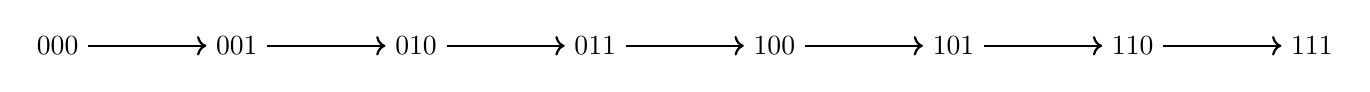
\begin{tikzpicture}[node distance=1.5cm, auto]
	% Nodes arranged in lexicographic order for 3-bit strings
	\node (000) {000};
	\node (001) [right=of 000] {001};
	\node (010) [right=of 001] {010};
	\node (011) [right=of 010] {011};
	\node (100) [right=of 011] {100};
	\node (101) [right=of 100] {101};
	\node (110) [right=of 101] {110};
	\node (111) [right=of 110] {111};
	
	% Arrows representing the ordering
	\draw[->, thick] (000) -- (001);
	\draw[->, thick] (001) -- (010);
	\draw[->, thick] (010) -- (011);
	\draw[->, thick] (011) -- (100);
	\draw[->, thick] (100) -- (101);
	\draw[->, thick] (101) -- (110);
	\draw[->, thick] (110) -- (111);
\end{tikzpicture}
\end{center}
\end{example*}

\newpage
\defbox[Maximal and Minimal]{\begin{definition*}
Let $(P,\preceq)$ be a poset. 
\begin{enumerate}[(1)]
	\item An element $m\in P$ is said to be \hl{\textbf{maximal}} in $P$ if \[
	\forall a\in P,\quad (m\preceq a)\implies(m=a).
	\] In other words, there exits no element in $P$ that is strictly greater than $m$.
	\item An element $m\in P$ is said to be \hl{\textbf{minimal}} in $P$ if \[
	\forall a\in P,\quad (a\preceq m)\implies(a=m).
	\] That is, there is no element in $P$ that is strictly less than $m$.
\end{enumerate}
\end{definition*}}

\begin{example*}
Consider the set \[
S=\set{2,3,4,6,9, 12}\subseteq\N
\] with the partial order defined by \textit{divisibility} (\ie, $x\preceq y\iff x\mid y$). See the Hasse diagram:
\begin{center}
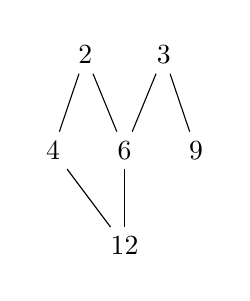
\begin{tikzpicture}
	\matrix (A) [matrix of nodes, row sep=.75cm]
	{ 
		  & 2 &    & 3 & \\  
		4 &   & 6  &   & 9 \\
		  &   & 12 &   & \\
	};
	\draw (A-1-2)--(A-2-1);
	\draw (A-1-2)--(A-2-3);
	\draw (A-1-4)--(A-2-3);
	\draw (A-1-4)--(A-2-5);
	\draw (A-2-1)--(A-3-3);
	\draw (A-2-3)--(A-3-3);
\end{tikzpicture}\hspace{20pt}
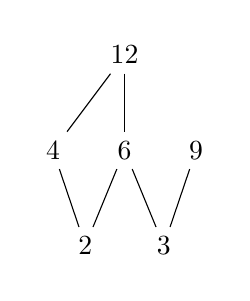
\begin{tikzpicture}
	\matrix (A) [matrix of nodes, row sep=.75cm]
	{ 
		&  &  12  &  & \\  
		4 &   & 6  &   & 9 \\
		& 2  & & 3  & \\
	};
	\draw (A-1-3)--(A-2-1);
	\draw (A-1-3)--(A-2-3);
	\draw (A-2-1)--(A-3-2);
	\draw (A-2-3)--(A-3-2);
	\draw (A-2-3)--(A-3-4);
	\draw (A-2-5)--(A-3-4);
\end{tikzpicture}
\end{center}
In this example, the minimal elements here are: $\set{2,3}$.
\end{example*} 
\begin{example*}
Consider the power set of $\set{a,b}$ with the usual subset relation $\subseteq$. The poset is \[
\set{\varnothing,\set{a},\set{b},\set{a,b}},
\] partially ordered by ``is a subset of.''
\begin{center}
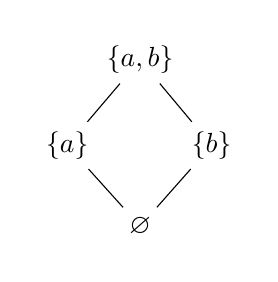
\begin{tikzpicture}
	\matrix (A) [matrix of nodes, row sep=.5cm]
	{ 
		&$\set{a,b}$&\\
		$\set{a}$ & & $\set{b}$\\
		&$\varnothing$& \\
	};
	\draw (A-1-2)--(A-2-1);
	\draw (A-1-2)--(A-2-3);
	\draw (A-2-1)--(A-3-2);
	\draw (A-2-3)--(A-3-2);
\end{tikzpicture}
\end{center}
\begin{itemize}
	\item The \textit{minimal element} here is $\varnothing$ (there's nothing strictly smaller).
	\item The \textit{maximal element} here is $\set{a,b}$ (there's nothing strictly bigger).
\end{itemize}
\end{example*}

\newpage
\defbox[Chain]{\begin{definition*}
	Let $(P,\preceq)$ be a poset. A subset $\mathcal{C}\subseteq P$ is called a \hl{\textbf{chain}} if \[
	\forall a,b\in \mathcal{C},\quad\text{either}\ a\preceq b\ \text{or}\ b\preceq a.
	\] In other words, a chain in a poset is a subset in which every two elements are comparable (\ie the subset is totally ordered).
\end{definition*}}
\begin{example*}
Consider a poset \[
P=\set{1,2,3,4,5,6,8,15}\subseteq\N
\] with the partial order defined by divisibility. See the Hasse diagram:
\begin{center}
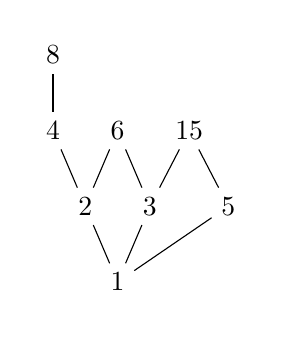
\begin{tikzpicture}
	\matrix (A) [matrix of nodes, row sep=.5cm]
	{ 
		8& \\
		4&   & 6 &   & 15 &\\
		& 2 &   & 3 &    &5\\
		&   & 1 &\\
	};
	\draw (A-4-3)--(A-3-2);
	\draw (A-4-3)--(A-3-4);
	\draw (A-4-3)--(A-3-6);
	\draw (A-3-2)--(A-2-1);
	\draw (A-3-2)--(A-2-3);
	\draw (A-3-4)--(A-2-3);
	\draw (A-3-4)--(A-2-5);
	\draw (A-3-6)--(A-2-5);
	\draw (A-2-1)--(A-1-1);
\end{tikzpicture}\hspace{40pt}
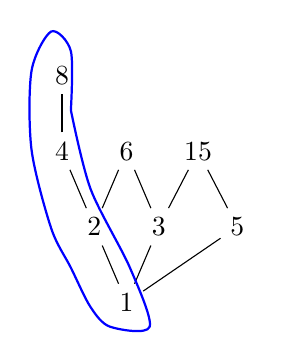
\begin{tikzpicture}
	\matrix (A) [matrix of nodes, row sep=.5cm]
	{ 
		8& \\
		4&   & 6 &   & 15 &\\
		& 2 &   & 3 &    &5\\
		&   & 1 &\\
	};
	\draw (A-4-3)--(A-3-2);
	\draw (A-4-3)--(A-3-4);
	\draw (A-4-3)--(A-3-6);
	\draw (A-3-2)--(A-2-1);
	\draw (A-3-2)--(A-2-3);
	\draw (A-3-4)--(A-2-3);
	\draw (A-3-4)--(A-2-5);
	\draw (A-3-6)--(A-2-5);
	\draw (A-2-1)--(A-1-1);
	\draw[color=blue,thick,smooth] plot coordinates {(-1,1) (-.75,0) (-.25,-1) (0,-1.75) (-.5, -1.75) (-.75,-1.5) (-1,-1) (-1.25,-.5) (-1.5, .5) (-1.5,1.5) (-1.25, 2) (-1,1.75) (-1,1)};
\end{tikzpicture}
\end{center}
Here, $\mathcal{C}=\set{1,2,4,8}$ is a \textit{chain} under divisibility.
\end{example*}
\hfill
\begin{example*}
Let $S=\set{a,b,c}$. Consider all the subsets of $S$ under the subset relation $\subseteq$. The entire power set of $S$ is \[
2^S=\set{\varnothing,\set{a},\set{b},\set{c},\set{a,b},\set{a,c},\set{b,c},\set{a,b,c}}.
\] This set $2^S$ (the power set) is partially ordered by $\subseteq$: for any $A,B\in 2^S$, \[
A\preceq B\iff A\subseteq B.
\]
\begin{center}
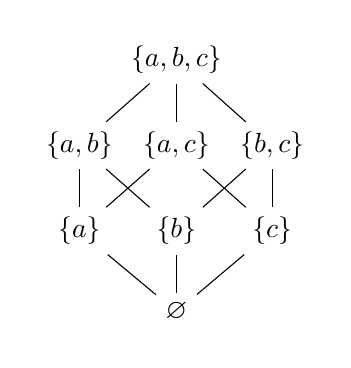
\begin{tikzpicture}
	\matrix (A) [matrix of nodes, row sep=.5cm]
	{ 
		&$\set{a,b,c}$&\\
		$\set{a,b}$ & $\set{a,c}$   & $\set{b,c}$\\
		$\set{a}$   & $\set{b}$     & $\set{c}$\\
		            & $\varnothing$ &\\
	};
\draw (A-4-2)--(A-3-1);
\draw (A-4-2)--(A-3-2);
\draw (A-4-2)--(A-3-3);
\draw (A-3-1)--(A-2-1);
\draw (A-3-1)--(A-2-2);
\draw (A-3-2)--(A-2-1);
\draw (A-3-2)--(A-2-3);
\draw (A-3-3)--(A-2-2);
\draw (A-3-3)--(A-2-3);
\draw (A-2-1)--(A-1-2);
\draw (A-2-2)--(A-1-2);
\draw (A-2-3)--(A-1-2);
\end{tikzpicture}\hspace{40pt}
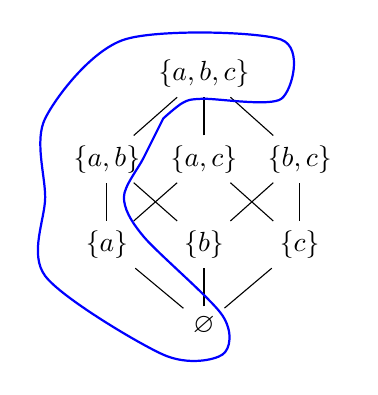
\begin{tikzpicture}
\matrix (A) [matrix of nodes, row sep=.5cm]
{ 
	&$\set{a,b,c}$&\\
	$\set{a,b}$ & $\set{a,c}$   & $\set{b,c}$\\
	$\set{a}$   & $\set{b}$     & $\set{c}$\\
	& $\varnothing$ &\\
};
\draw (A-4-2)--(A-3-1);
\draw (A-4-2)--(A-3-2);
\draw (A-4-2)--(A-3-3);
\draw (A-3-1)--(A-2-1);
\draw (A-3-1)--(A-2-2);
\draw (A-3-2)--(A-2-1);
\draw (A-3-2)--(A-2-3);
\draw (A-3-3)--(A-2-2);
\draw (A-3-3)--(A-2-3);
\draw (A-2-1)--(A-1-2);
\draw (A-2-2)--(A-1-2);
\draw (A-2-3)--(A-1-2);
	\draw[color=blue,thick,smooth] plot coordinates {(-.5,1) (-.75,.5) (-1,0) (-.75,-.5) (.25, -1.5) (.25,-2) (-.5,-2) (-2,-1) (-2, 0) (-2, 1) (-1, 2) (1,2) (1,1.25) (0,1.25) (-.25,1.2) (-.5,1)};
\end{tikzpicture}
\end{center}
Here, $\mathcal{C}=\set{\varnothing,\set{a},\set{a,b},\set{a,b,c}}$ is a \textit{chain} in $2^S$.
\end{example*}

\newpage
\axiombox[Zorn's Lemma]{\begin{axiom*}
	Let $(P,\preceq)$ be a nonempty partially ordered set with property that every chain $C\subseteq P$ has an upper bound in $P$; that is, for every chain $C\subseteq P$, \[
	\exists u\in P\quad \text{such that}\quad \forall c\in C,\quad c\preceq u.
	\] Then $P$ contains at least one maximal element; that is, \[
	\exists m\in P\quad\text{such that}\quad\forall a\in P,\quad (m\preceq a)\implies(m=a).
	\]
\end{axiom*}}
%\begin{proof}
%	See \hyperlink{zorn}{Proof of Zorn's Lemma}.
%\end{proof}

\vfill
\begin{observation}[Existence of Basis] Let $\mathcal{L}:=\set{S\subseteq \R^3:S\ \text{is linearly independent}}$.
\ \begin{center}
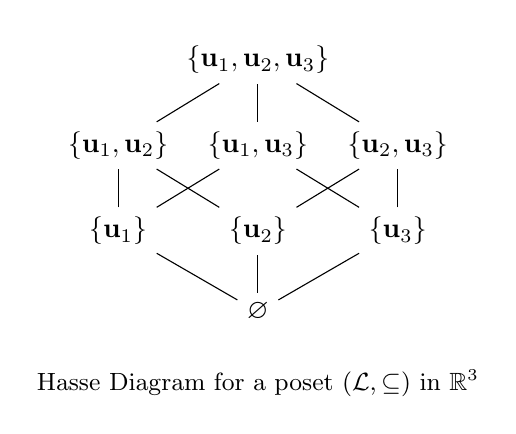
\begin{tikzpicture}
	\matrix (A) [matrix of nodes, row sep=.5cm]
	{ 
		&$\set{\vec{u}_1,\vec{u}_2,\vec{u}_3}$&\\
		$\set{\vec{u}_1,\vec{u}_2}$&$\set{\vec{u}_1,\vec{u}_3}$&$\set{\vec{u}_2,\vec{u}_3}$\\
		$\set{\vec{u}_1}$& $\set{\vec{u}_2}$ &$\set{\vec{u}_3}$\\
		& $\varnothing$ &\\
	};
	\draw (A-4-2)--(A-3-1);
	\draw (A-4-2)--(A-3-2);
	\draw (A-4-2)--(A-3-3);
	\draw (A-3-1)--(A-2-1);
	\draw (A-3-1)--(A-2-2);
	\draw (A-3-2)--(A-2-1);
	\draw (A-3-2)--(A-2-3);
	\draw (A-3-3)--(A-2-2);
	\draw (A-3-3)--(A-2-3);
	\draw (A-2-1)--(A-1-2);
	\draw (A-2-2)--(A-1-2);
	\draw (A-2-3)--(A-1-2);
	\node[draw=none, below=.25cm of A] {\small Hasse Diagram for a poset \((\mathcal{L},\subseteq)\) in \(\mathbb{R}^3\)};
\end{tikzpicture}\hspace{40pt}
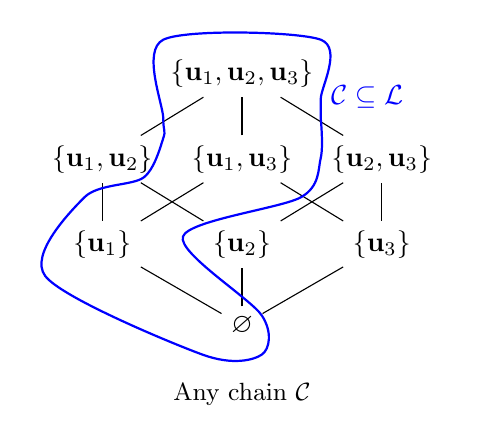
\begin{tikzpicture}
	\matrix (A) [matrix of nodes, row sep=.5cm]
	{ 
		&$\set{\vec{u}_1,\vec{u}_2,\vec{u}_3}$&\\
		$\set{\vec{u}_1,\vec{u}_2}$&$\set{\vec{u}_1,\vec{u}_3}$&$\set{\vec{u}_2,\vec{u}_3}$\\
		$\set{\vec{u}_1}$& $\set{\vec{u}_2}$ &$\set{\vec{u}_3}$\\
		& $\varnothing$ &\\
	};
	\draw (A-4-2)--(A-3-1);
	\draw (A-4-2)--(A-3-2);
	\draw (A-4-2)--(A-3-3);
	\draw (A-3-1)--(A-2-1);
	\draw (A-3-1)--(A-2-2);
	\draw (A-3-2)--(A-2-1);
	\draw (A-3-2)--(A-2-3);
	\draw (A-3-3)--(A-2-2);
	\draw (A-3-3)--(A-2-3);
	\draw (A-2-1)--(A-1-2);
	\draw (A-2-2)--(A-1-2);
	\draw (A-2-3)--(A-1-2);
	\node[draw=none, below=.25cm of A] {\small Any chain $\mathcal{C}$};
	
	\draw[color=blue,thick,smooth] plot coordinates {(1,1) (1,.5) (.75,0) (-.75,-.5) (.25, -1.5) (.25,-2) (-.5,-2) (-2.5,-1) (-2, 0) (-1.25,.25) (-1,.75) (-1, 1) (-1, 2) (1,2) (1,1.25) (1,1)} node[above right] {$\mathcal{C}\subseteq\mathcal{L}$};
\end{tikzpicture}
\end{center}
\begin{center}
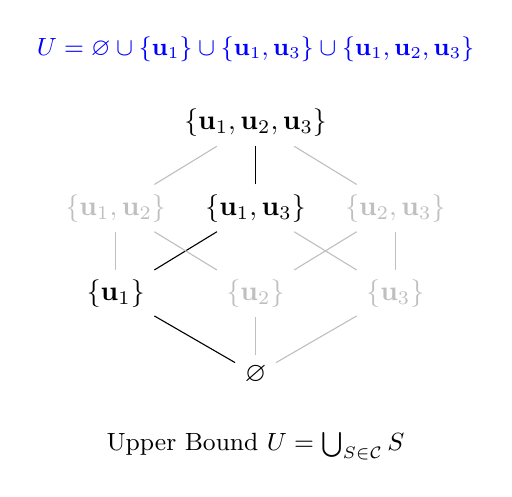
\begin{tikzpicture}
	\matrix (A) [matrix of nodes, row sep=.5cm]
	{ 
		&$\set{\vec{u}_1,\vec{u}_2,\vec{u}_3}$&\\
		\color{gray!50}$\set{\vec{u}_1,\vec{u}_2}$&$\set{\vec{u}_1,\vec{u}_3}$&\color{gray!50}$\set{\vec{u}_2,\vec{u}_3}$\\
		$\set{\vec{u}_1}$& \color{gray!50}$\set{\vec{u}_2}$ &\color{gray!50}$\set{\vec{u}_3}$\\
		& $\varnothing$ &\\
	};
	\draw (A-4-2)--(A-3-1);
	\draw[gray!50] (A-4-2)--(A-3-2);
	\draw[gray!50] (A-4-2)--(A-3-3);
	\draw[gray!50] (A-3-1)--(A-2-1);
	\draw (A-3-1)--(A-2-2);
	\draw[gray!50] (A-3-2)--(A-2-1);
	\draw[gray!50] (A-3-2)--(A-2-3);
	\draw[gray!50] (A-3-3)--(A-2-2);
	\draw[gray!50] (A-3-3)--(A-2-3);
	\draw[gray!50] (A-2-1)--(A-1-2);
	\draw (A-2-2)--(A-1-2);
	\draw[gray!50] (A-2-3)--(A-1-2);
	\node[draw=none, below=.25cm of A] {\small Upper Bound \(U=\bigcup_{S\in\mathcal{C}}S\)};
	\node[blue] at (0,2.5) {\small $U=\varnothing\cup\set{\vec{u}_1}\cup\set{\vec{u}_1,\vec{u}_3}\cup\set{\vec{u}_1,\vec{u}_2,\vec{u}_3}$};
\end{tikzpicture}\hspace{40pt}
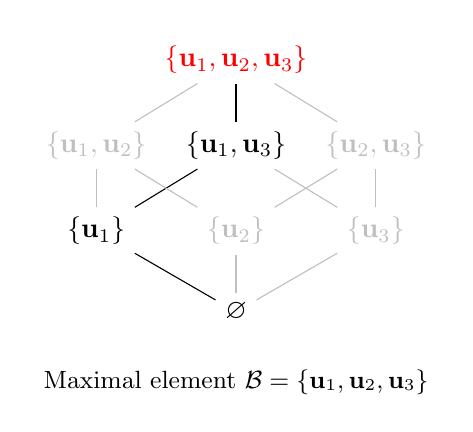
\begin{tikzpicture}
	\matrix (A) [matrix of nodes, row sep=.5cm]
	{ 
		&\color{red}$\set{\vec{u}_1,\vec{u}_2,\vec{u}_3}$&\\
		\color{gray!50}$\set{\vec{u}_1,\vec{u}_2}$&$\set{\vec{u}_1,\vec{u}_3}$&\color{gray!50}$\set{\vec{u}_2,\vec{u}_3}$\\
		$\set{\vec{u}_1}$& \color{gray!50}$\set{\vec{u}_2}$ &\color{gray!50}$\set{\vec{u}_3}$\\
		& $\varnothing$ &\\
	};
	\draw (A-4-2)--(A-3-1);
	\draw[gray!50] (A-4-2)--(A-3-2);
	\draw[gray!50] (A-4-2)--(A-3-3);
	\draw[gray!50] (A-3-1)--(A-2-1);
	\draw (A-3-1)--(A-2-2);
	\draw[gray!50] (A-3-2)--(A-2-1);
	\draw[gray!50] (A-3-2)--(A-2-3);
	\draw[gray!50] (A-3-3)--(A-2-2);
	\draw[gray!50] (A-3-3)--(A-2-3);
	\draw[gray!50] (A-2-1)--(A-1-2);
	\draw (A-2-2)--(A-1-2);
	\draw[gray!50] (A-2-3)--(A-1-2);
	\node[draw=none, below=.25cm of A] {\small Maximal element $\mathcal{B}=\set{\vec{u}_1,\vec{u}_2,\vec{u}_3}$};
\end{tikzpicture}
\end{center}	
\end{observation}

\newpage
\thmbox[$\star$ Hamel Basis Theorem $\star$]{\begin{theorem*}
	Every vector space $V$ over a field $F$ has a basis.
\end{theorem*}}
\begin{proof}
\ \begin{flushleft}\color{red}
\textbf{Key Idea}: ``By considering all linearly independent subsets of \(V\) and partially ordering them by inclusion, we use \underline{Zorn's Lemma} to guarantee a maximal linearly independent set exists.''
\end{flushleft}
\begin{enumerate}[Step 1]
	\item \textbf{Definition of Poset.}
	
	Define the set \[
	\mathcal{L}:=\set{S\subseteq V:\text{$S$ is linearly independent}}.
	\] with the partial order $\preceq$ on $\mathcal{L}$ by set inclusion: \[
	\forall S,T\in\mathcal{L},\quad S\preceq T\iff S\subseteq T.
	\] Since $\varnothing\in\mathcal{L}$, we have $\mathcal{L}\neq\varnothing$. Thus, $(\mathcal{L},\subseteq)$ forms a poset.
	\item \textbf{Chains and Upper Bounds.}
	
	Let $\mathcal{C}\subseteq\mathcal{L}$ be any chain, \ie, \[
	\forall S,T\in\mathcal{C},\quad S\subseteq T\ \text{or}\ T\subseteq S.
	\] Now, we need to find an upper bound $U\in\mathcal{L}$ of $\mathcal{C}$. Define \[
	U:=\bigcup_{S\in\mathcal{C}}S.
	\] Clearly, $U\subseteq V$. We claim that $U$ is linearly independent, \ie, $U\in\mathcal{L}$:
	\begin{enumerate}
		\item[] (\textit{Proof of $U\in\mathcal{L}$})\quad Let $n\in\N$ and suppose \[
		a_1\vec{u}_1+a_2\vec{u}_2+\cdots+a_n\vec{u}_n=0\quad\text{with}\ a_i\in F, \vec{u}_i\in U\ \text{for}\ i=1,2,\dots,n.
		\] Since $U=\bigcup_{S\in\mathcal{C}}S$, \[
		\vec{u}_i\in U\iff \exists S_i\in\mathcal{C}\ \text{such that}\ \vec{u}_i\in S_i
		\] for each $i\in\set{1,2,\dots,n}$. Since $\mathcal{C}$ is a chain (totally ordered by inclusion), the sets $S_1,S_2,\dots,S_n$ are comparable. Therefore, there exists at least one set $S^*\in\mathcal{C}$ such that \[
		(\forall i\in\set{1,2,\dots,n},\ \vec{u}_i\in S^*)\quad\ie,\quad\set{\vec{u}_1,\vec{u}_2,\dots,\vec{u}_n}\subseteq S^*.
		\] Since $S^*$ is an element of $\mathcal{C}$ (and $\mathcal{C}\subseteq\mathcal{L}$, where every element is linearly independent), the linear independence of $S^*$ implies that \[
		a_1=a_2=\cdots=a_n=0.
		\] Thus, $U$ is linearly independent, \ie, $U\in\mathcal{L}$.
	\end{enumerate}
	 By definition of $U$, we know \[
	 \forall S\in\mathcal{C},\ S\subseteq U,
	 \] and so $U\in\mathcal{L}$ be an upper bound of $\mathcal{C}$.
	\item \textbf{Application of Zorn's Lemma.}
	
	Since every chain $\mathcal{C}$ in $\mathcal{L}$ has an upper bound $U\in\mathcal{L}$, Zorn's Lemma guarantees the existence of a maximal element $\mathcal{B}\in\mathcal{L}$ such that \[
	\forall S\in\mathcal{L},\ (\mathcal{B}\subseteq S)\implies (\mathcal{B}=S),\quad\ie,\quad\nexists S\in\mathcal{L}\ \text{with}\ \mathcal{B}\subseteq S.
	\]
	\item \textbf{$\mathcal{B}$ is a Basis of $V$.}
	
	We now show that $\mathcal{B}$ spans $V$, \ie, $\Span\mathcal{B}=V$. Assume, for contradiction, that \[
	\Span\mathcal{B}\neq V,\quad\ie,\quad\exists\vec{v}_0\in V\setminus\Span\mathcal{B}.
	\] Consider \[
	\mathcal{B}'=\mathcal{B}\cup\set{\vec{v}_0}.
	\] We NTS that $\mathcal{B}'$ is linearly independent. Suppose that for $n\in\N$, scalars $a_0,a_1,\cdots,a_n\in F$ and distinct vectors $\vec{v}_0,\vec{b}_1,\vec{b}_2,\cdots,\vec{b}_n\in\mathcal{B}'$, the followings holds: \[
	a_0\vec{v}_0+(a_1\vec{b}_1+a_2\vec{b}_2+\cdots+a_n\vec{b}_n)=0.
	\] \begin{enumerate}[(\text{Case} I)]
		\item If $a_0=0$, then \[
		a_1\vec{b}_1+a_2\vec{b}_2+\cdots+a_n\vec{b}_n=0
		\] and since $\mathcal{B}$ is linearly independent, $a_i=0$ for $i=1,2,\dots, n$.
		\item If $a_0\neq 0$, then \[
		\vec{v}_0=-\frac{1}{a_0}(a_1\vec{b}_1+a_2\vec{b}_2+\cdots+a_n\vec{b}_n)\in\Span\mathcal{B},
		\] which contradicts the assumption that $\vec{v}_0\notin\Span\mathcal{B}$.
	\end{enumerate}
	Thus, in all cases, \[
	a_0=a_1=\cdots=a_n=0.
	\] Hence, $\mathcal{B}'$ is linearly independent, \ie, $\mathcal{B}'\in\mathcal{L}$, and $\mathcal{B}\subseteq\mathcal{B}'$, contradicting the maximality of $\mathcal{B}$.
\end{enumerate}

\end{proof}
\begin{remark*}
	This theorem and its proof is a classic demonstration of how abstract set-theoretic principles can yield concrete and essential results in linear algebra.
\end{remark*}
\vspace{40pt}
\defbox{\begin{definition*}
Consider any two sets $S_1$ and $S_2$. \begin{enumerate}[(1)]
	\item (Equal Cardinalities) We write \[
	\abs{S_1}=\abs{S_2}
	\] if and only if there exists a bijective (one-to-one and onto) function $f:S_1\to S_2$.
	\item (Strict Inequality of Cardinalities) We write \[
	\abs{S_1} <\abs{S_2}
	\] if and only if there exists an injective (one-to-one) function $f:S_1\to S_2$ but no bijective function from $S_1$ onto $S_2$ exists.
\end{enumerate}
\end{definition*}}
\begin{center}
\begin{minipage}{.49\textwidth}\centering
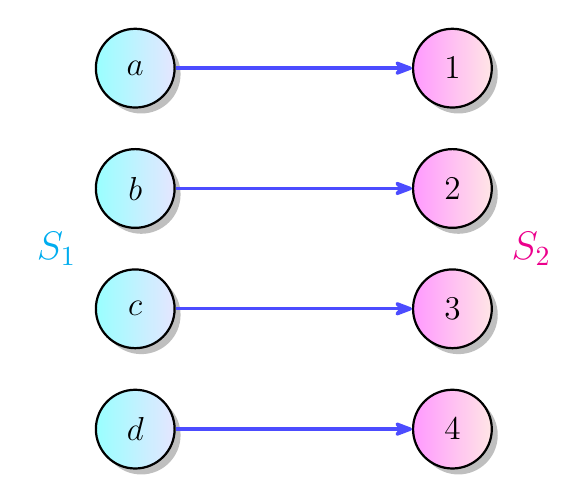
\begin{tikzpicture}[>=Stealth, auto, node distance=1cm,
	% Define styles for nodes and arrows
	set1node/.style={circle, draw, minimum size=1cm, font=\large, drop shadow, 
		shade, shading=radial, left color=cyan!40, right color=blue!10, thick},
	set2node/.style={circle, draw, minimum size=1cm, font=\large, drop shadow, 
		shade, shading=radial, left color=magenta!40, right color=red!10, thick},
	arrow style/.style={-{Stealth[round]}, very thick, blue!70},
	label style/.style={font=\Large\bfseries}
	]
	% Nodes for set S_1
	\node[set1node] (s1-1) {$a$};
	\node[set1node, below=.5cm of s1-1] (s1-2) {$b$};
	\node[set1node, below=.5cm of s1-2] (s1-3) {$c$};
	\node[set1node, below=.5cm of s1-3] (s1-4) {$d$};
	
	% Nodes for set S_2
	\node[set2node, right=3cm of s1-1] (s2-1) {1};
	\node[set2node, right=3cm of s1-2] (s2-2) {2};
	\node[set2node, right=3cm of s1-3] (s2-3) {3};
	\node[set2node, right=3cm of s1-4] (s2-4) {4};
	
	% Set labels
	\node[label style, cyan] at ($(s1-1)!0.5!(s1-4) + (-1,0)$) {$S_1$};
	\node[label style, magenta] at ($(s2-1)!0.5!(s2-4) + (1,0)$) {$S_2$};
	
	% Draw bijection arrows
	\draw[arrow style] (s1-1) -- (s2-1);
	\draw[arrow style] (s1-2) -- (s2-2);
	\draw[arrow style] (s1-3) -- (s2-3);
	\draw[arrow style] (s1-4) -- (s2-4);
\end{tikzpicture}
\end{minipage}\hfill
\begin{minipage}{.49\textwidth}\centering
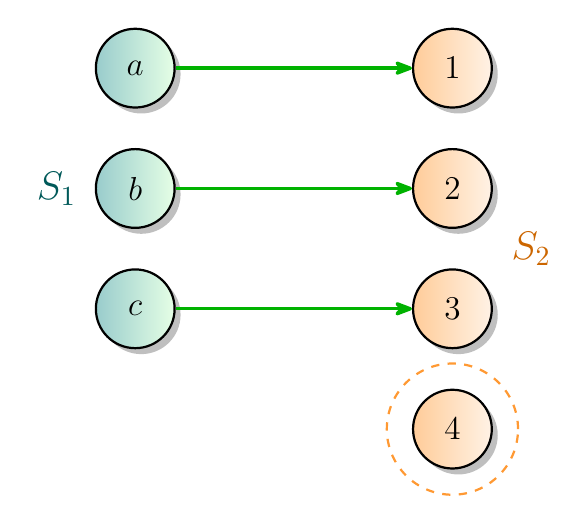
\begin{tikzpicture}[>=Stealth, auto, node distance=1cm,
	% Define styles for nodes and arrows
	set1node/.style={circle, draw, minimum size=1cm, font=\large, drop shadow, 
		shade, shading=radial, left color=teal!40, right color=green!10, thick},
	set2node/.style={circle, draw, minimum size=1cm, font=\large, drop shadow, 
		shade, shading=radial, left color=orange!40, right color=orange!10, thick},
	arrow style/.style={-{Stealth[round]}, very thick, green!70!black},
	label style/.style={font=\Large\bfseries}
	]
	% Nodes for the smaller set S_1
	\node[set1node] (s1-1) {$a$};
	\node[set1node, below=.5cm of s1-1] (s1-2) {$b$};
	\node[set1node, below=.5cm of s1-2] (s1-3) {$c$};
	
	% Nodes for the larger set S_2
	\node[set2node, right=3cm of s1-1] (s2-1) {1};
	\node[set2node, right=3cm of s1-2] (s2-2) {2};
	\node[set2node, right=3cm of s1-3] (s2-3) {3};
	\node[set2node, below=.5cm of s2-3] (s2-4) {4};
	
	% Set labels
	\node[label style, teal!70!black] at ($(s1-1)!0.5!(s1-3) + (-1,0)$) {$S_1$};
	\node[label style, orange!80!black] at ($(s2-1)!0.5!(s2-4) + (1,0)$) {$S_2$};
	
	% Draw injection arrows (from S_1 to a subset of S_2)
	\draw[arrow style] (s1-1) -- (s2-1);
	\draw[arrow style] (s1-2) -- (s2-2);
	\draw[arrow style] (s1-3) -- (s2-3);
	
	% Emphasize the unmapped element in S_2
	\node[draw=orange!80, thick, dashed, circle, fit=(s2-4), inner sep=.75mm] {};
\end{tikzpicture}
\end{minipage}
\end{center}

\newpage
\lembox[Steinitz's Exchange Lemma]{\begin{lemma*}
Let $V$ be a vector space over a field $F$. Suppose that \begin{enumerate}[(i)]
	\item $\mathcal{X}=\set{\vec{x}_1,\vec{x}_2,\dots,\vec{x}_m}\subseteq V$ is a linearly independent set, and
	\item $\mathcal{Y}=\set{\vec{y}_1,\vec{y}_2,\dots,\vec{y}_n}\subseteq V$ is a spanning set of $V$, \ie, $\Span\mathcal{Y}=V$.
\end{enumerate}	Then \[
\abs[1]{\mathcal{X}} \;\leq\; \abs[1]{\mathcal{Y}},
\] that is, there exists an injective function $f:\mathcal{X}\rightarrowtail\mathcal{Y}$.
\end{lemma*}}
\begin{proof}
	TBA	
\end{proof}
\vspace{20pt}
\thmbox[Invariance of Basis Cardinality]{\begin{theorem*}
	Let $V$ be a vector space over a field $F$, and let $\mathcal{B}_1$ and $\basis_2$ be two bases of $V$. Then \[
	\abs{\basis_1}=\abs{\basis_2}.
	\]
\end{theorem*}}
\begin{proof}
Suppose, for the contradiction, that \[
\abs{\basis_1}<\abs{\basis_2}.
\] Since $\basis_1$ is a basis, it spans $V$. Also since $\basis_2$ is a basis, it is linearly independent. Applying the Steinitz's Exchange Lemma, we obtain \[
\abs{\basis_2}\leq\abs{\basis_1}\quad\text{\large\lightning}.
\] Thus, it is not possible to have bases $\basis_1$ and $\basis_2$ of $V$ with different cardinalities.
\end{proof}
\vspace{40pt}\newpage
\defbox[Dimension of Vector Space]{\begin{definition*}
	Let $V$ be a vector space over a field $F$. The \hl{\textbf{dimension}} of $V$, denoted by $\dim V$, is defined as the cardinality of any basis $\basis$ of $V$: \[
	\dim V:=\abs\basis.
	\] 
\end{definition*}}
\begin{remark*}
By the Invariance of Basis Cardinality, this definition does not depend on the choice of the basis.
\end{remark*}

\vfill
\begin{thebibliography}{9}
	\bibitem{linear_algebra_1}
	수학의 즐거움, Enjoying Math. ``수학 공부, 기초부터 대학원 수학까지, 14. 선형대수학 (a) 벡터공간의 정의와 초른의 보조정리'' YouTube Video, 27:20. Published 
	October 8, 2019. URL: \url{https://www.youtube.com/watch?v=esLn0FeedyQ}.
	\bibitem{linear_algebra_2}
	수학의 즐거움, Enjoying Math. ``수학 공부, 기초부터 대학원 수학까지, 15. 선형대수학 (b) 벡터공간의 기저의 존재성과 차원'' YouTube Video, 24:41. Published 
	October 10, 2019. URL: \url{https://www.youtube.com/watch?v=oGC_BU5Erkk&t=875s}.
	\bibitem{SteinitzExchangeLemma}
	Wikipedia, The Free Encyclopedia. ``Steinitz exchange lemma.'' Wikipedia Article. Accessed February 25, 2025. URL: \url{https://en.wikipedia.org/wiki/Steinitz_exchange_lemma}.
\end{thebibliography}

%\newpage
%\appendix
%\section{Proof of Zorn's Lemma from Axiom of Choice}
%\thmbox{\begin{theorem*}\hypertarget{zorn}{}
%The following statements are equivalent: \begin{enumerate}
%	\item \textbf{Axiom of Choice (AC)}:\quad For every indexed family $\set{S_i}_{i\in I}$ of nonempty sets, there exists a choice function $f:I\to\bigcup_{i\in I}S_i$ such that $f(i)\in X_i$ for all $i\in I$.
%	\item \textbf{Zorn's Lemma}:\quad If $(P,\preceq)$ is a nonempty partially ordered set in which every chains has an upper bound in $P$, then $P$ contains at least one maximal element.
%\end{enumerate}
%\end{theorem*}}
%\begin{proof}
%\begin{itemize}
%	\item[($\Rightarrow$)] $(\textbf{AC}\implies \textbf{ZL})$ Assume that the Axiom of Choice holds.
%	\begin{enumerate}
%		\item \textbf{Definition of Poset}
%		
%		Let $(P,\preceq)$ be a nonempty partially ordered set with the property that every chain in $P$ has an upper bound in  $P$.
%		
%		\item \textbf{Construction of an Extending Function}
%		
%		Define the family $\set{\mathcal{C}_i}_{i\in I}$ of chains in $P$. For any chain $\mathcal{C}_i$ that is not maximal with respect to inclusion (\ie, $\exists $), AC guarantees that we can elect an element \[
%		f(C)
%		\] 
%	\end{enumerate}
%	\item[($\Leftarrow$)] $(\textbf{ZL}\implies \textbf{AC})$ 
%\end{itemize}
%\end{proof}
\end{document}
